\documentclass{article}
\usepackage[margin = .7in]{geometry}
\usepackage[dvipdfmx]{graphicx}
\usepackage{listings}
\usepackage{amsmath}
\usepackage{bm}
\lstset{%
  language={python},
  basicstyle={\small},%
  identifierstyle={\small},%
  commentstyle={\small\itshape},%
  keywordstyle={\small\bfseries},%
  ndkeywordstyle={\small},%
  stringstyle={\small\ttfamily},
  frame={tb},
  breaklines=true,
  columns=[l]{fullflexible},%
  numbers=left,%
  xrightmargin=0zw,%
  xleftmargin=3zw,%
  numberstyle={\scriptsize},%
  stepnumber=1,
  numbersep=1zw,%
  lineskip=-0.5ex%
}

\begin{document}
\title{STAT6011/7611/6111/3317 \\ 
COMPUTATIONAL STATISTICS (2016 Fall) \\
Assignment 3}
\author{Kei Ikegami (u3535947)}
\maketitle

\section{}
	\subsection{}
		\begin{align*}
			p({\bf y} | \sigma^2) &= \idotsint \Pi_{i = 1}^{n} \frac{1}{\sqrt{2\pi}} \exp\left( -\frac{(y_i - \theta_i)^2}{2}\right)\frac{1}{\sqrt{2\pi}\sigma} \exp\left( -\frac{\theta_i^2}{2\sigma^2}\right)\mathrm{d}\theta_1 \dots \mathrm{d}\theta_n \\
			&= \idotsint \Pi_{i = 1}^{n} \frac{1}{\sqrt{2\pi}\sqrt{\sigma^2 + 1}} \exp\left( -\frac{y_i}{2} + \frac{\sigma^2 y_i^2}{2(\sigma^2 + 1)}\right) \frac{\sqrt{\sigma^2 + 1}}{\sqrt{2\pi}\sigma} \exp\left( \frac{\sigma^2 + 1}{\sigma^2} \left(\theta_i -\frac{\sigma^2}{\sigma^2 + 1}y_i \right)\right)\mathrm{d}\theta_1 \dots \mathrm{d}\theta_n \\
			&= \Pi_{i = 1}^{n} \frac{1}{\sqrt{2\pi}\sqrt{\sigma^2 + 1}} \exp\left( -\frac{y_i}{2} + \frac{\sigma^2 y_i^2}{2(\sigma^2 + 1)}\right) \\
			&= \left(\frac{1}{\sqrt{2\pi}\sqrt{\sigma^2 + 1}}\right)^{n} \exp \left( -\frac{\sum_{i=1}^{n} y_i}{2} + \frac{\sigma^2 \sum_{i=1}^{n} y_i^2}{2(\sigma^2 + 1)}\right)
		\end{align*}
	\subsection{}
		\begin{align*}
			p(\sigma^2 | {\bf y}) \propto \left(\frac{1}{\sqrt{2\pi}\sqrt{\sigma^2 + 1}}\right)^{n} \exp \left( -\frac{\sum_{i=1}^{n} y_i}{2} + \frac{\sigma^2 \sum_{i=1}^{n} y_i^2}{2(\sigma^2 + 1)}\right) \frac{1}{\sigma^2}
		\end{align*}
		\lstinputlisting[caption=1-b]{1-b.py}
		\begin{center}
		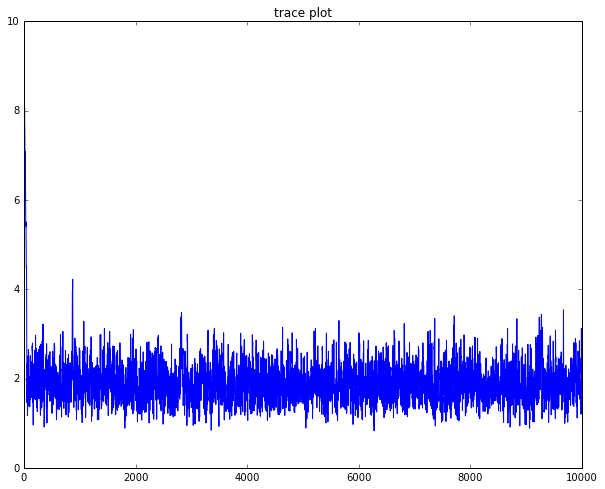
\includegraphics[width = 12cm]{1-b.png}
		\end{center}
	\subsection{}
	Let $\Theta = (\theta_1, \theta_2, \dots , \theta_n)$, and let $\Theta_{-j} = (\theta_1, \dots, \theta_{j-1}, \theta_{j+1}, \dots, \theta_n)$.
		\begin{align*}
			p(\sigma^2 | {\bf y}, \Theta) &\propto \frac{1}{\sigma^2(\sqrt{2\pi \sigma^2})^n} \exp\left( -\frac{\sum_i^n \theta_i^2}{2\sigma^2}\right) \\
			p(\theta_j | {\bf y}, \Theta_{-j}, \sigma^2) &\propto N \left( \frac{\sigma^2 y_j}{\sigma^2 + 1}, \frac{\sigma^2}{\sigma^2 + 1}\right) \forall j \in \left\{1, 2, 3, \dots, n \right\} \\
		\end{align*}
		\lstinputlisting[caption=1-c]{1-c.py}
		Trace plot. $\sigma^2$ and $\theta_1$.
		\par
		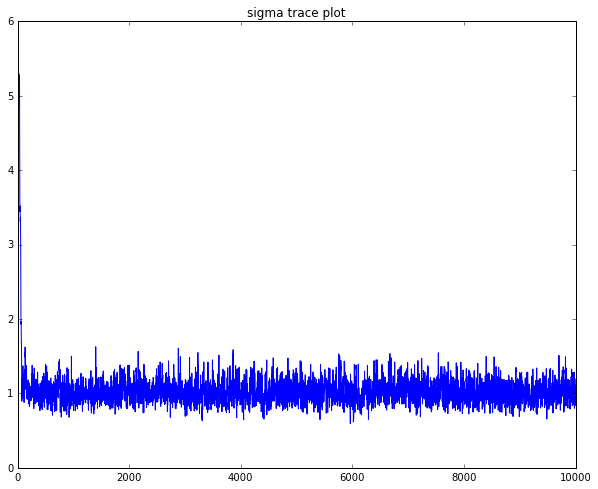
\includegraphics[width = 9cm]{1-c-sigma.png}
		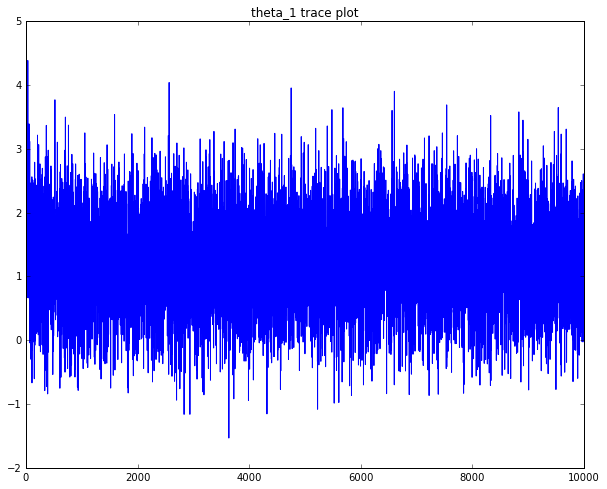
\includegraphics[width = 9cm]{1-c-theta.png}
		
	
\section{}
	\subsection{}
		\begin{align*}
		p({\bf y} | \sigma^2) &= \idotsint \Pi_{i = 1}^{n} \left(\Pi_{j=1}^{J} \frac{1}{\sqrt{2\pi}} \exp\left( -\frac{(y_{ij} - \theta_i)^2}{2}\right) \right)\frac{1}{\sqrt{2\pi}\sigma} \exp\left( -\frac{\theta_i^2}{2\sigma^2}\right)\mathrm{d}\theta_1 \dots \mathrm{d}\theta_n \\
		&= \idotsint \Pi_{i = 1}^{n} \exp\left( -\frac{\sum_{j=1}^{J} y_{ij}^2}{2} + \frac{\sigma^2 (\sum_{j=1}^{J} y_{ij})^2}{2(\sigma^2 + 1)} \right) \frac{1}{\sqrt{2\pi}^J} \frac{1}{\sqrt{J\sigma^2 + 1}} \\ &\frac{\sqrt{J\sigma^2 + 1}}{\sqrt{2\pi}\sigma} \exp\left(-\frac{J\sigma^2 + 1}{2\sigma^2} \left( \theta_i - \frac{\sigma^2}{J\sigma^2 + 1} \sum_{j=1}^{J} y_{ij} \right)^2\right)\mathrm{d}\theta_1 \dots \mathrm{d}\theta_n \\
		&= \Pi_{i=1}^{n} \frac{1}{\sqrt{2\pi}^J} \frac{1}{\sqrt{J\sigma^2 + 1}} \exp\left( -\frac{\sum_{j=1}^{J} y_{ij}^2}{2} + \frac{\sigma^2 (\sum_{j=1}^{J} y_{ij})^2}{2(\sigma^2 + 1)} \right)\\
		&= \frac{1}{\sqrt{2\pi}^{nJ}} \frac{1}{\sqrt{J\sigma^2 + 1}^{n}} \exp\left( -\frac{\sum_{i=1}^{n} \sum_{j=1}^{J} y_{ij}^2}{2} + \frac{\sigma^2 \sum_{i=1}^{n} \left( \sum_{j=1}^{J} y_{ij}\right)^2}{2(J\sigma^2+ 1)}\right)\\
		\end{align*}
	\subsection{}
		We prove the marginal likelihood is bounded away from 0 around the neighborhood of $\sigma^2 = 0$. In such a case, the usual prior, like Jaffrey's prior, which has infinite mass on the neighborhood, leads to an improper posterior distribution, because the multiplication of prior and the likelihood results in infinite among the neighbor hood. 
		\par
		First, we calculate the first derivative of the marginal likelihood function with respect to $\sigma^2$, and will show that in the support of $\sigma^2$ the function is monotone decreasing function when $n \neq 1$ and $J \neq 1$. Let L be the part of marginal likelihood function concerning with $\sigma^2$.
		\begin{align}
			L(\sigma^2) &= (J\sigma^2 + 1)^{-\frac{n}{2}} \exp \left( \frac{\sigma^2}{J\sigma^2 + 1}\right) \nonumber \\
			\frac{\partial L}{\partial \sigma^2} &= \exp \left( \frac{\sigma^2}{J\sigma^2 + 1} \right) (J \sigma^2 + 1)^{-\frac{n}{2}-2}\left( 1 - \frac{nJ^2}{2}\sigma^2 - \frac{nJ}{2}\right)
		\end{align}
		Since $\sigma^2 > 0$, $J\sigma^2 +1$ can not be equal to 0. Thus,
		\begin{align*}
			&\frac{\partial L(\sigma^2)}{\partial \sigma^2} = 0
			\Leftrightarrow 1- \frac{nJ^2}{2}\sigma^2 - \frac{nJ}{2} = 0
			\Leftrightarrow \sigma^2 = \frac{2 - nJ}{nJ^2}
		\end{align*}
		Since $n > 0, J >0$, 
		\begin{align*}
			\begin{cases}
			\frac{2 - nJ}{nJ^2} > 0 \Rightarrow 2 > nJ \\
			\frac{2 - nJ}{nJ^2} \le 0 \Rightarrow 2 \le nJ
			\end{cases}
		\end{align*}
		In other words, the function has it extreme value in its support when both of n and J is equal to 1, and does not have otherwise. 
		In the former case, 
		\begin{align*}
			\frac{\partial L(0)}{\partial \sigma^2} = 1 - \frac{nJ}{2} = \frac{1}{2}
		\end{align*}
		the fact that we can calculate the first derivative at $\sigma^2 = 0$ implies that the function is continuous at the point. Then the marginal likelihood function is increasing function until it reaches its extreme value. Thus there is some neighborhood around $\sigma^2 = 0$ among which the function value is lower bounded by 1, that is bigger than 0. So we are done with this case.
		\par
		In the latter case, 
		\begin{align*}
			\frac{\partial L(0)}{\partial \sigma^2} = 1 - \frac{nJ}{2} \leq 0
		\end{align*}
		By (1), we know the first derivative is negative when $\sigma^2 > 0$, and so the function is decreasing in this case. As the same as the previous case, the function is continuous as $\sigma^2 = 0$ since the first derivative exists at $\sigma^2 = 0$. Due to the definition of continuity of function, we can take some neighborhood around $\sigma = 0$ where the value generated by the function is included in $[1 - \epsilon, 1]$  for any $\epsilon > 0$. 1 is the limit of the marginal likelihood function as $\sigma^2 \to 0$. This means we can take the neighborhood around $\sigma^2 = 0$ whose value is lower bounded by some positive number.
		By the above two part, we prove the function is lower bounded away from 0. So we are done.
	\subsection{}
	By problem 2-a, we can derive the below posterior distribution.
		\begin{align*}
		p(\sigma^2 | {\bf y}) &\propto \frac{1}{\sigma^2} \frac{1}{\sqrt{J\sigma^2 + 1}^n} \exp \left( \frac{\sigma^2 \sum_{i=1}^{n} \left( \sum_{j=1}^{J} y_{ij}\right)^2}{2(J\sigma^2+ 1)}\right)
		\end{align*}
		\lstinputlisting[caption=2-c]{2-c.py}
		\begin{center}
		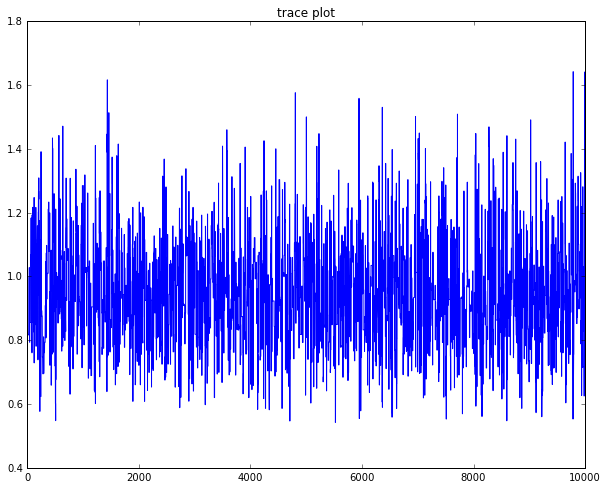
\includegraphics[width = 12cm]{2-c.png}
		\end{center}		
	\subsection{}
	Use the previous notations. And by the same way we get the below posterior distributions.
		\begin{align*}
			p(\sigma^2 | \Theta, {\bf y}) &\propto \frac{1}{\sigma^2 \sqrt{2\pi\sigma^2}^n} \exp \left( -\frac{\sum_{i=1}^{n} \theta_{i}^{2}}{2\sigma^2}\right)\\
			p(\theta_i | \Theta_{-i}, {\bf y}, \sigma^2) &\propto N\left( \frac{\sigma^2 \sum_{j=1}^{J} y_{ij}}{1 + J\sigma^2}, \frac{\sigma^2}{1 + J\sigma^2}\right) \forall i \in \left\{ 1,2,3, \dots, n \right\} \\
		\end{align*}
		\lstinputlisting[caption=2-d]{2-d.py}
		\par
		Trace plot. $\sigma^2$ and $\theta_1$.
		\par
		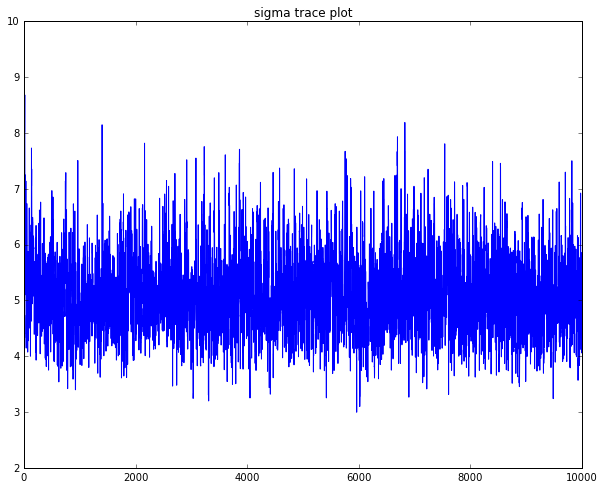
\includegraphics[width = 9cm]{2-d-sigma.png}
		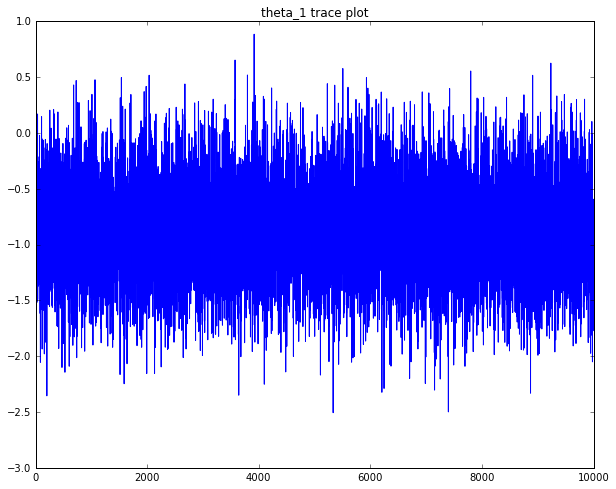
\includegraphics[width = 9cm]{2-d-theta.png}

\section{}
	\subsection{}
	Let $\hat{\beta} = ({\bf X}^T{\bf X})^{-1}{\bf X}^T{\bf y}$ and $\hat{\epsilon} = {\bf y}-\hat{{\bf y}}$.
		\begin{align*}
		p(\beta, \sigma^2 | {\bf X}, {\bf y}) &\propto \frac{1}{\sigma^2} p({\bf y} | {\bf X}, \beta, \sigma^2) \\
		&\propto (\sigma^2)^{-(\frac{n}{2} +1)} \exp\left( \frac{1}{2\sigma^2} ({\bf y} - {\bf X}\beta)^T ({\bf y} - {\bf X}\beta)\right)\\
		&= (\sigma^2)^{-(\frac{n}{2} +1)} \exp\left( \frac{1}{2\sigma^2} (\hat{\epsilon}^T\hat{\epsilon} + (\beta - \hat{\beta})^T ({\bf X}^T{\bf X})(\beta - \hat{\beta}) )\right)\\
		\end{align*}
	\subsection{}
	Let $\theta = \frac{2}{\hat{\epsilon}^T\hat{\epsilon} + (\beta - \hat{\beta})^T ({\bf X}^T{\bf X})(\beta - \hat{\beta}) )}$
		\begin{align*}
		p(\beta | {\bf X}, {\bf y}) &= \int \left( \frac{1}{\sigma^2}\right)^{\frac{n}{2} + 1} \exp \left( \frac{1}{\sigma^2 \theta}\right) \mathrm{d} \sigma^2
		= \int |\sigma^{-4}| \left(\frac{1}{\sigma^2} \right)^{\frac{n}{2} + 1} \exp \left( \frac{1}{\sigma^2 \theta}\right) \mathrm{d} \sigma^{-2}\\
		&= \int \left(\frac{1}{\sigma^2} \right)^{\frac{n}{2} -1} \exp \left( \frac{1}{\sigma^2 \theta}\right) \mathrm{d} \sigma^{-2}
		= \Gamma \left(\frac{n}{2} \right) \theta^{\frac{n}{2}} \int \frac{1}{\Gamma(\frac{n}{2})} \left(\frac{1}{\theta}\right)^{\frac{n}{2}} \left( \frac{1}{\sigma^2}\right)^{\frac{n}{2} -1} \exp \left( \frac{1}{\sigma^2 \theta}\right) \mathrm{d} \sigma^{-2}\\
		&= \Gamma \left(\frac{n}{2} \right) \left(\frac{1}{\theta} \right)^{-\frac{n}{2}}
		\propto \left(\frac{1}{\theta} \right)^{-\frac{n}{2}}\\
		&= \left( \frac{\hat{\epsilon}^T\hat{\epsilon}}{2} \frac{\hat{\epsilon}^T\hat{\epsilon} + (\beta - \hat{\beta})^T ({\bf X}^T{\bf X})(\beta - \hat{\beta}))}{\hat{\epsilon}^T\hat{\epsilon}}\right)^{-\frac{n}{2}}
		\propto \left( 1 + \frac{(\beta - \hat{\beta})^T ({\bf X}^T{\bf X})(\beta - \hat{\beta}))}{\hat{\epsilon}^T\hat{\epsilon}}\right)^{-\frac{n}{2}}\\
		\end{align*}
		\par 
		This means the posterior distribution of $\beta$ is $t_{n-k} (\hat{\beta} , S_{\epsilon}^2({\bf X}^T{\bf X})^{-1})$, where $S_{\epsilon}^2 = \frac{\hat{\epsilon}^T\hat{\epsilon}}{n-k}$.
		\par
		Next we calculate the posterior distribution of $\sigma^2$.
		\begin{align*}
			p(\sigma^2 | {\bf X}, {\bf y}) &= \int (\sigma^2)^{-(\frac{n}{2} + 1)} \exp\left( -\frac{\hat{\epsilon}^T\hat{\epsilon} + (\beta - \hat{\beta})^T ({\bf X}^T{\bf X})(\beta - \hat{\beta})}{2\sigma^2}\right) \mathrm{d} \beta\\
			&= (2\pi)^{\frac{n}{2}} |\left(\frac{{\bf X}^T{\bf X}}{\sigma^2}\right)^{-1}| (\sigma^2)^{-(\frac{n}{2} + 1)} \exp\left( -\frac{\hat{\epsilon}^T\hat{\epsilon}}{2\sigma^2}\right) \\ &\int \frac{1}{(2\pi)^{\frac{n}{2}} |\left(\frac{{\bf X}^T{\bf X}}{\sigma^2}\right)^{-1}|} \exp\left( -\frac{1}{2} \left( (\beta - \hat{\beta})^T ((\frac{{\bf X}^T {\bf X}}{\sigma^2})^{-1})^{-1} (\beta - \hat{\beta})\right)\right) \mathrm{d} \beta \\
			&= \frac{(2\pi)^{\frac{n}{2}}}{|{\bf X}^T{\bf X}|}(\sigma^2)^{-\frac{n}{2}} \exp\left( -\frac{\hat{\epsilon}^T\hat{\epsilon}}{2\sigma^2}\right)\\
			&\propto (\sigma^2)^{-\frac{n}{2}} \exp\left( -\frac{\hat{\epsilon}^T\hat{\epsilon}}{2\sigma^2}\right)\\
		\end{align*}
		The last term tells us that the posterior distribution of $\sigma^2$ is inverse gamma distribution whose parameters are $(\frac{n}{2}, \frac{\hat{\epsilon}^T\hat{\epsilon}}{2})$.
		Thus, the posterior mean of $\beta$ is $\hat{\beta}$ and one of $\sigma^2$ is $\frac{\frac{\hat{\epsilon}^T\hat{\epsilon}}{2}}{\frac{n}{2} -1} = \frac{\hat{\epsilon}^T\hat{\epsilon}}{n-2}$.
	
	
	
	
	
	
\end{document}
















